\begin{problem}{Little H And Reboot}{standard input}{standard output}{5 seconds}{256 megabytes}

One day, HZNU Online Judge server was unable to log in, resulting in Hsueh- unable to upload problems on the server.

After hard judgment, Hsueh- guessed that this was because the server was down.


Poor Hsueh- just go to the machine room and restart the server.

After a long period of time, Hsueh- finally found the computer room and found the location of the server, but he had never seen this super non-quantum low-speed potato server from Pangalactic Universe Invincible Co., Ltd., and didn't know how to restart it. .

Recalling that when I bought this server before, a master came to install it, and I never shut it down once.

This left him helpless. He could only call the master, but the master also forgot how to operate.

Finally, the master told him that the manual had been thrown in a certain position in the warehouse and told him the coordinates. Now Hsueh- can finally find a way to restart the server!

When Hsueh- walked into the warehouse, he found that due to the random stacking before, the whole warehouse was very chaotic. Even if he knew the coordinates, he needed to go over some boxes.

Because the boxes are randomly placed, they will not overlap.

For instance, the warehouse might look like the picture below. It can be considered that the warehouse is infinitely large, and Hsueh- is infinitely small, which can be regarded as a point.

\begin{center}
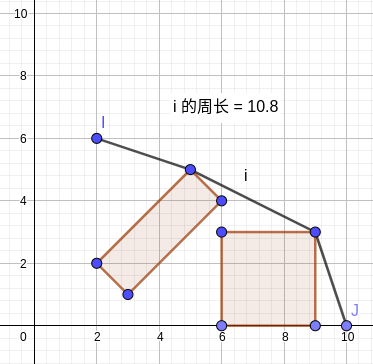
\includegraphics[width=8cm,height=10cm,natwidth=320,natheight=360]{data1.png} % 插入图片
\end{center}


Since the box was moved around all day, plus a lot of roads, he finally didn't want to climb over, so he decided to bypass the box. At the same time, he hopes to take the shortest path.

However, he wants you to tell him the shortest path length, so that he can decide whether to restart the server or replace it with a Pangalactic Universe Invincible Infinite Co., Ltd. Super Advanced Unspeakable Fairy Server.



\InputFile
The first line contains a single integer $n(0 \leq n \leq 200)$, denoting the number of boxes in the warehouse.

Next $n$ lines, each line $8$ integers, $x_{i_0},y_{i_0},x_{i_1},y_{i_1},x_{i_2},y_{i_2},x_{i_3}, y_{i_3}$, arranged in a counterclockwise direction, representing a rectangular box.

The $n + 2$ line contains $4$ integers $x_0, y_0, x_1, y_1$, respectively representing the coordinates of Hsueh- and the coordinates of the manual.

The absolute value of all integers does not exceed $10000$.

Test data to ensure that the vertices of two boxes will not overlap, and at the same time ensure that the vertices of one box will not appear on the edge of the other box.


\OutputFile
Print a single float number, denoting your answer.

Your answer is considered correct if its absolute or relative error does not exceed $10^{-4}$.


Formally, let your answer be $a$, and the jury's answer be $b$. Your answer is accepted if and only if $\frac{|a - b|}{\max{(1, |b|)}} \le 10^{-4}$.



\Example

\begin{example}
\exmpfile{example.01}{example.01.a}%
\end{example}

\end{problem}

